\section{Scene Analysis and Synthesis}
\label{sec:scene}

The analysis of model collections has so far been prevalently focused on single objects,
where the main focus of study is the arrangement and relations between shape parts, and their
connection with functionality or semantics~\cite{Mitra:2014:SASP}.
Compared to the structure of shape parts in a single object, the structural layout of objects in a scene
is more complex due to the looser spatial relations and a more diverse mixture of functional substructures.

Scene understanding has been a well-studied problem in computer vision, with many specific tasks such as
recognition~\cite{quattoni2009}, classification~\cite{swadzba2010}, and
inferring spatial layout~\cite{Choi:2013:UIS} or other 3D information~\cite{Fouhey:2013:DDP} \emph{from a single image}.
With the rapid development of RGBD scans and availability of large repositories of 3D models,
2D scene understanding driven by 3D scans or models is becoming popular.
The key issue is how to relate the content in image to a large collection of 3D models,
to allow \emph{information transfer} from the models for a rich understanding of the input scene~\cite{Satkin:2012:DDS}.
The RGBD scans, coming with calibrated RGB image and depth information, can be used as training data for
establishing the link between 2D and 3D for model-driven scene understanding~\cite{Silberman:2012:ISS}.

In this section, we will mainly cover works on scene analysis and synthesis
from the graphics community, with the main focus on 3D indoor scenes.

\paragraph*{Context-based retrieval.}
Perhaps the first attempts on analyzing 3D scene collections were made by the serial of works of
Fisher et al.~\shortcite{Fisher:2010:CSM,Fisher:2011:CSR}.
Given a 3D scene database with semantic tags for objects, they learn the strength of spatial relationship
between pairs of objects using kernel density estimation~\cite{Fisher:2010:CSM}. Such learned spatial relationship
can be used in context-based object retrieval, which can be quite effective in assisting interactive scene modeling.
For example, the user places a bounding box into the partially modeled scene as a proxy and the system
can return a relevant object which both conforms to the size of the proxy and admits the contextual relationship against
the surrounding objects.
%
Later, Fisher et al. propose the first similarity measure for 3D scenes through
representing scenes as graphs which encode models and their contextual relationships and then
defining a kernel between the relationship graphs~\cite{Fisher:2011:CSR}.
Such graph kernel based scene similarity is shown to be discriminative for scene retrieval.
Meanwhile, since the graph kernel integrates spatial relationships between all objects in the scene,
it is also informative in characterizing contextual information and outperforms their previous method~\cite{Fisher:2010:CSM}
for context-based object retrieval.


%\teaser{
\begin{figure}[t]
\centering
    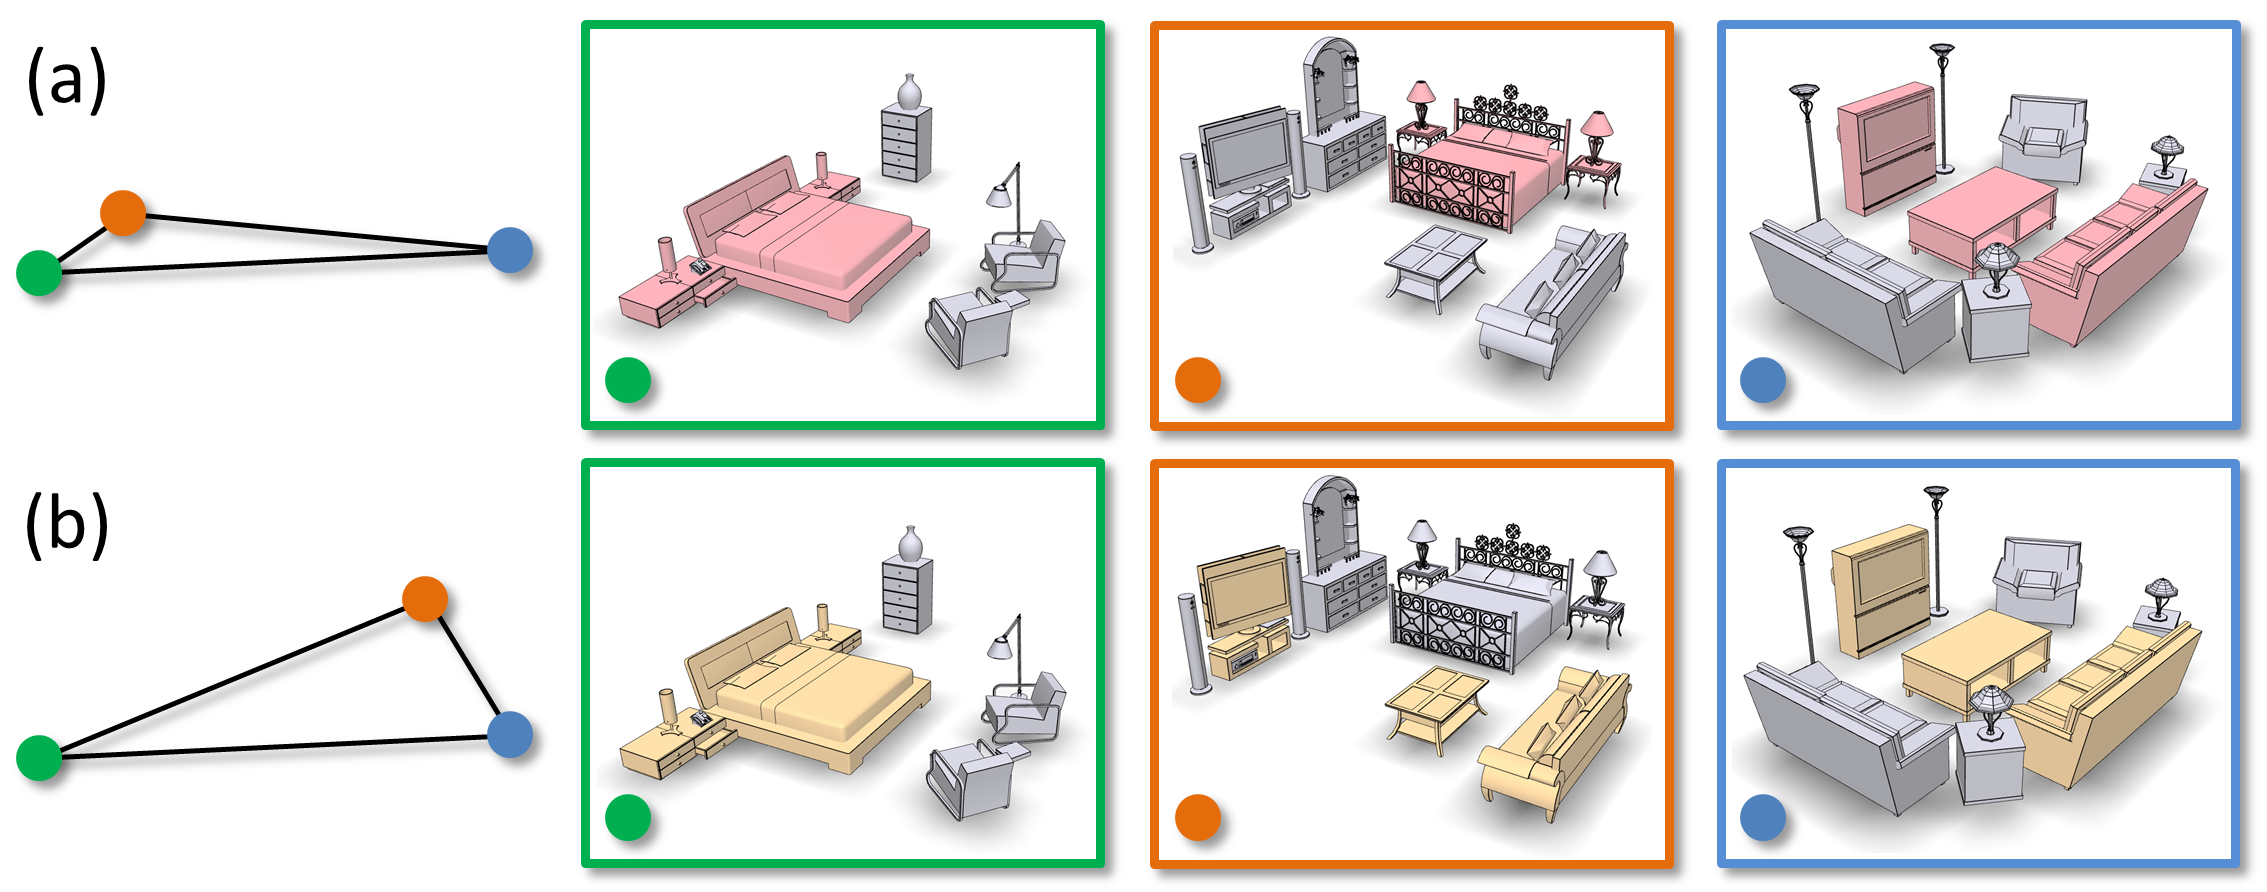
\includegraphics[width=0.99\linewidth]{fig/img/xu_sig14_focal}
    %\vspace{-0.2cm}
    \caption{
    Scene comparisons may yield different similarity distances (left) depending on the focal points~\cite{Xu:2014:OHSC}.}
    \label{fig:xu_sig14_focal}
\end{figure}
%}


\paragraph*{Contextual analysis.}
To co-analyze a collection of scenes, a central problem is to measure the similarity between the scenes.
This is especially challenging for those complex, hybrid scenes such as a studio composed
in part by bedroom, living room and dinning room.
The integral nature of graph kernel makes it only suited for measuring the global similarity,
obliterating the fine-grained similarity between complex scenes.
In the work of Xu et al.~\shortcite{Xu:2014:OHSC}, it is advocated that complex scenes should be compared
with respect to a focal point which is a subscene of the complex scene.
Figure~\ref{fig:xu_sig14_focal} shows an example of comparing two complex scenes, where the distance is not unique
depending on which subscene is focused on.

%In the work, focal points are determined within a context, via co-analyzing a set of scenes.
%Specifically, a focal point is defined as a subscene which can characterize a semantic scene category,
%i.e., frequently occurs only within that category.
%Therefore, focal point detection is naturally coupled with scene clustering.
In the work, a focal point is defined as a representative substructure of a specific scene category.
This requires that the substructure must occur frequently in that category.
Meanwhile, such representativity is tied to a notion of compactness of the group of scenes the focal
point is to represent or characterize. Therefore, frequency-based analysis is intermixed with clustering of the
scene collection, so that the scenes in each cluster are close when viewed from the perspective of the
representative focal points of the cluster.
%
The coupled problems are solved via interleaving optimization which interleaves between focal point detection
and focal-based scene clustering. The former is achieved by frequent substructure mining and the
latter adopts subspace clustering based on focal-centric scene distance computed with graph kernel.
%
The detected focal points can be used to organize the scene collection to support efficient exploration
of the collection (see Section~\ref{sec:exploration}).
Based on the focal points, they also derive a novel scene similarity called focal-centric graph kernel.
Such focal-based scene similarity can be used for novel applications such as multi-query scene retrieval
where one may issue queries consisting of multiple semantically related scenes and wish to retrieve more
scenes ``of the same''.% (Figure~\ref{fig:multiquery}).

%
\begin{figure}[t] \centering
    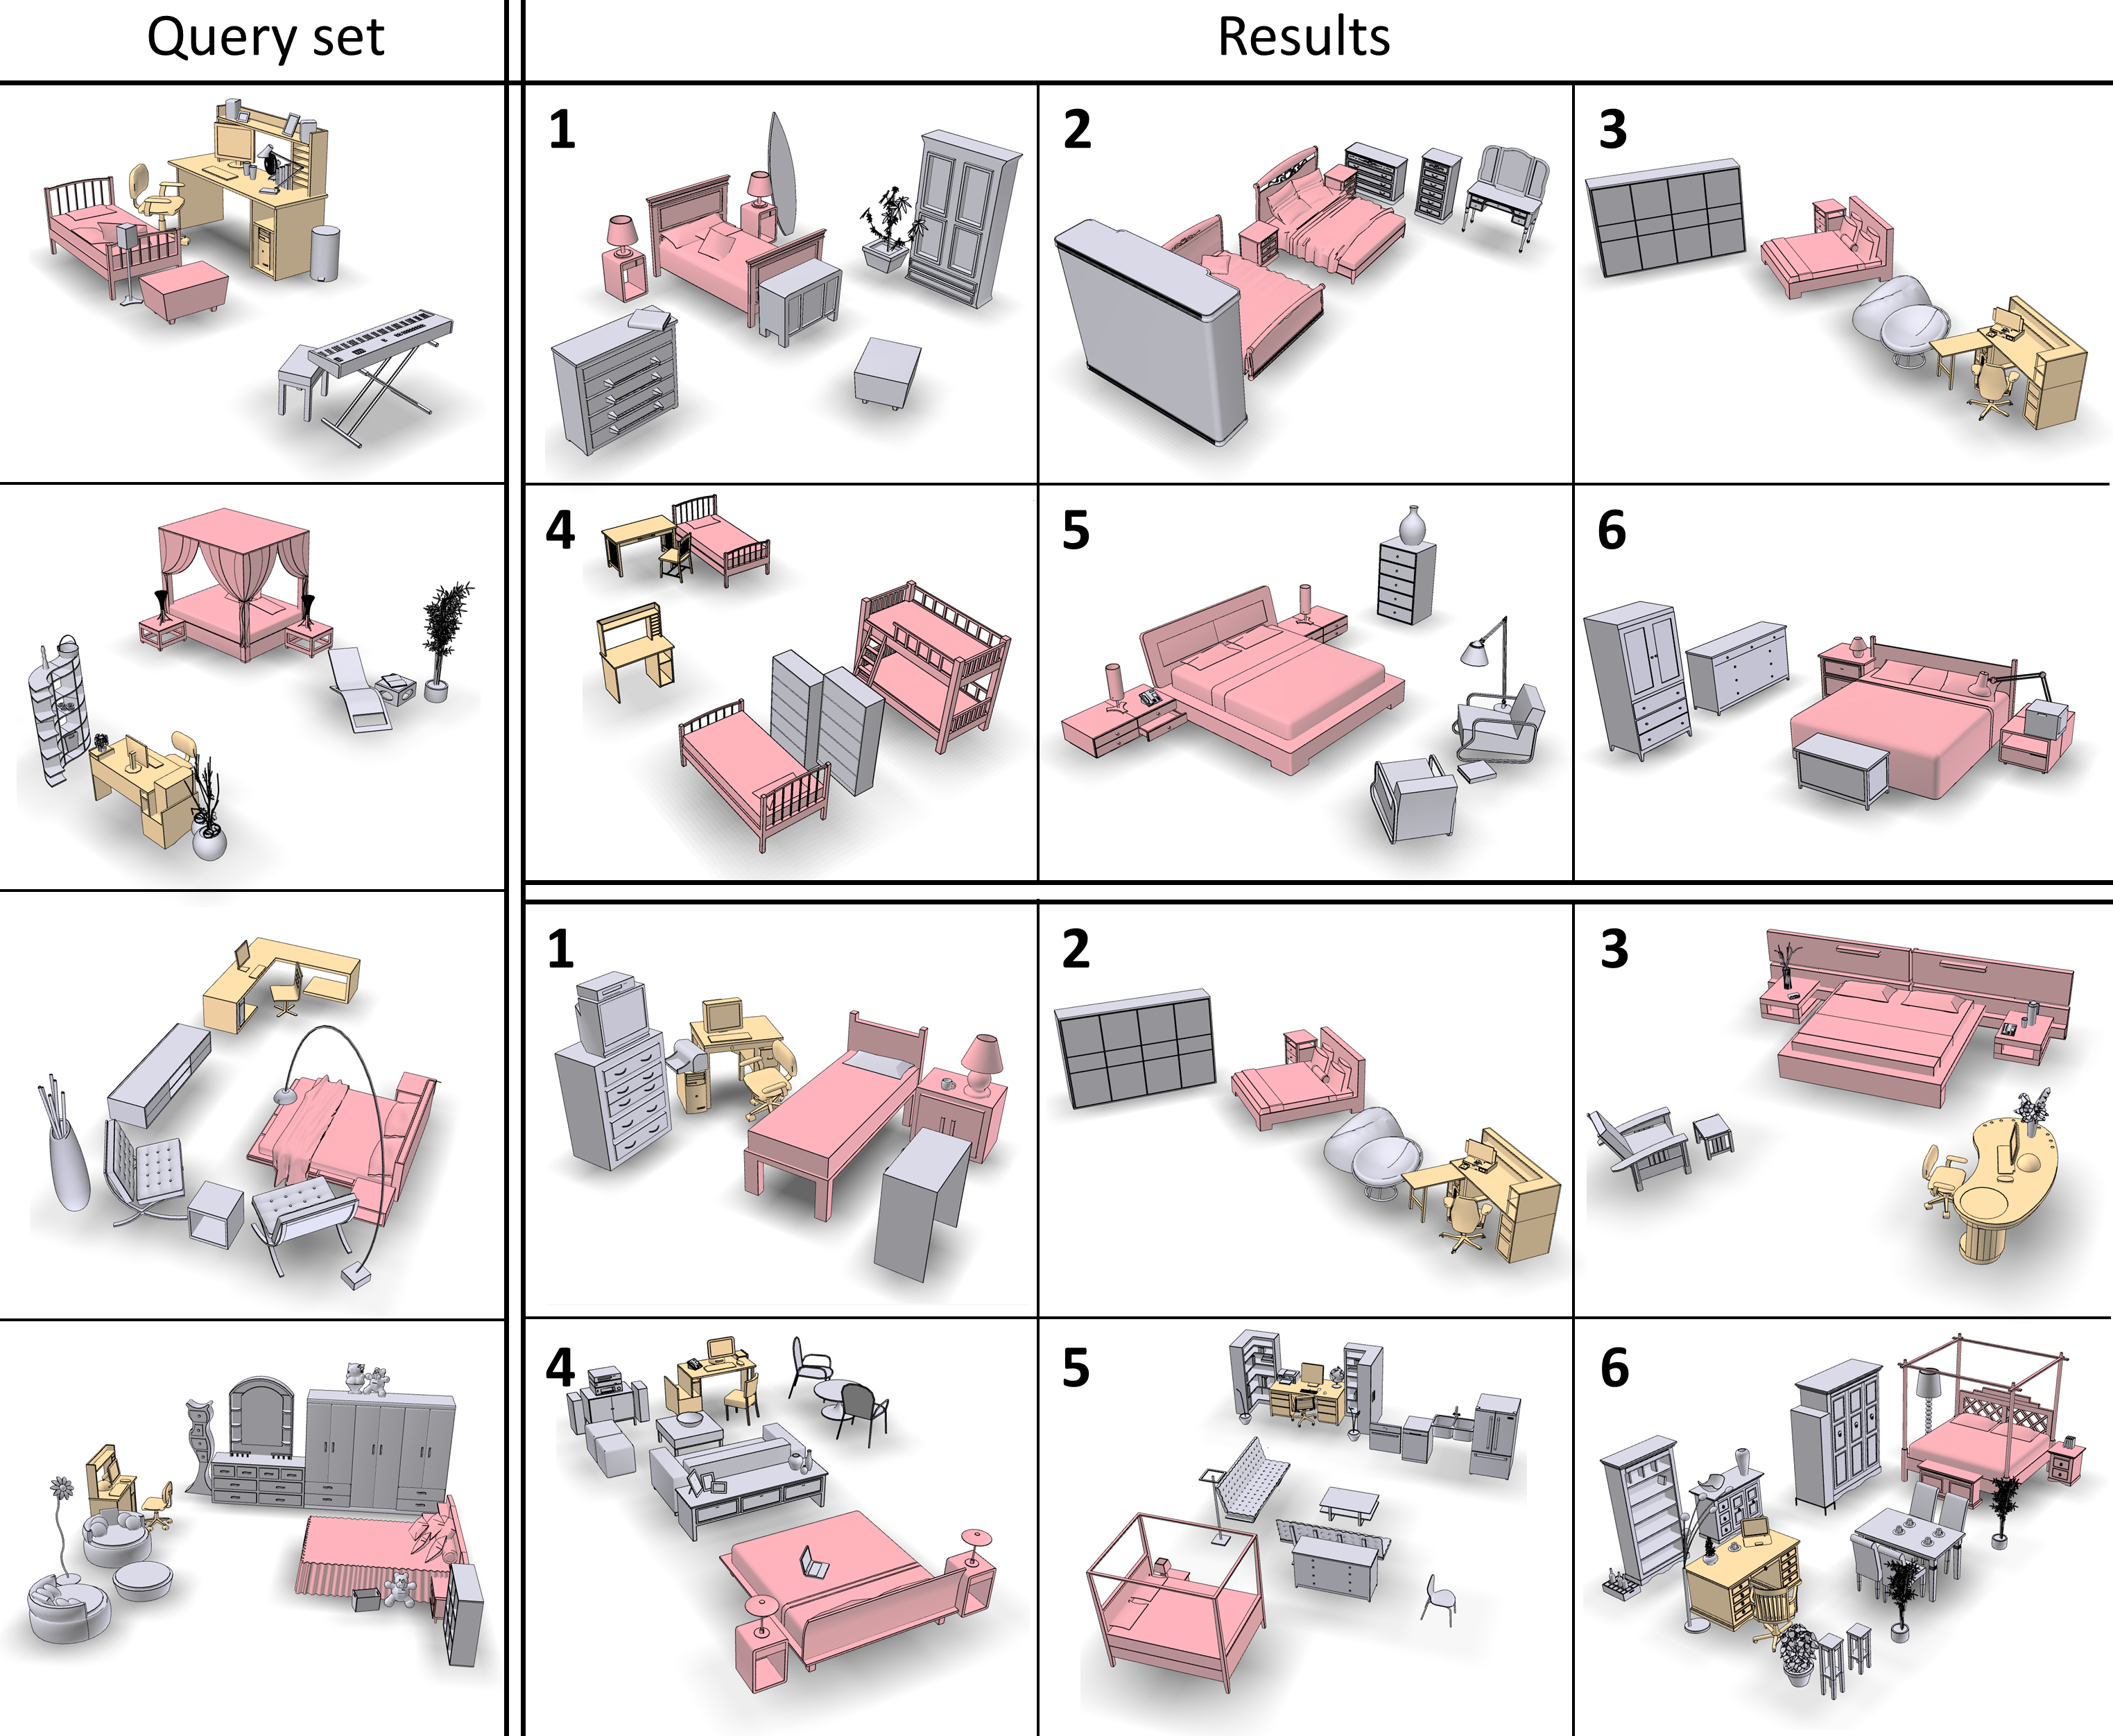
\includegraphics[width=0.98\linewidth]{fig/img/xu_sig14_multiquery}
        \vspace{-0.4cm}
    \caption{
    Multi-query retrieval takes a query set (left) and returns a ranked list of scenes (bottom-right) via focal (colored red and yellow) based scene comparison.
    Returns based on global scene similarity computed by graph kernel are also shown (top-right).
    }
    \vspace{-0.6cm}    
    \label{fig:multiquery}
\end{figure}


\paragraph*{Hierarchical analysis.}
Hierarchical decomposition graph is the most widely adopted representation for 3D scene models in industry.
Consistent scene hierarchies of a collection of semantically related scenes
reveals functional groupings of scene objects and encodes the knowledge about functional substructures of the input scenes.
Liu et al.~\shortcite{Liu:2014:CCS} proposed a supervised learning approach to the extraction of consistent
hierarchies for scene collections.
Given a collection of scene graphs with consistent hierarchies and labels, they train
a probabilistic hierarchical grammar encoding the distributions of shapes, cardinalities,
and spatial relationships of scene objects.
Such grammar can then be used to parse a new scene, so as to transfer the learned segmentations, labels, and hierarchies
consistent with the collection, onto the new scene; see Figure~\ref{fig:liu_siga14_sh}.


\begin{figure}[t] \centering
    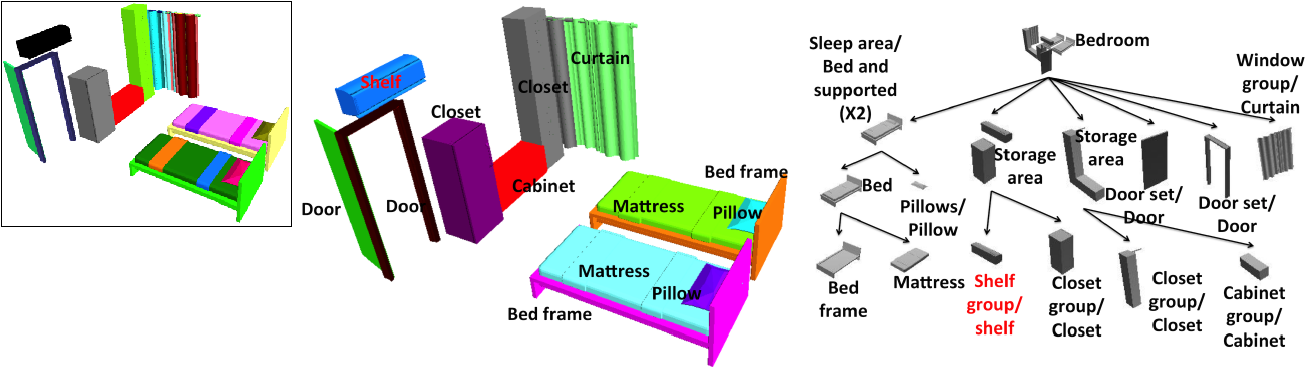
\includegraphics[width=0.98\linewidth]{fig/img/liu_siga14_sh}
        %\vspace{-0.3cm}
    \caption{
    The algorithm processes raw scene graphs with possible over-segmentation (a) into consistent hierarchies capturing semantic and functional groups (b,c)~\cite{Liu:2014:CCS}.
    }
    \label{fig:liu_siga14_sh}
\end{figure}


\paragraph*{Synthesis.}
With the knowledge about object occurrence and spatial layout learned from a database of scenes,
one can synthesize new scenes instantializing the knowledge.
Scene synthesis usually involves two basic models: object occurrence model based on context-based object retrieval
and object placement model via layout optimization.
Fisher et al.~\shortcite{Fisher:2012:CSR} proposed example-based, data-driven scene synthesis.
The method first learn the two synthesis models from a training database of 3D scenes.
Given an example scene, the method can generate similar scenes by populating with objects retrieved
from database and perform object layout through sampling the probabilistic model learned with database.
Xu et al.~\shortcite{Xu:2013:S2S} proposed modeling 3D indoor scenes from 2D sketches, which is supported
by a database of 3D scenes. They learn the contextual information
for both object occurrence and placement from the database.
Based on that, they perform sketch-guided co-retrieval of scene objects from the database,
as well as context-based co-placement of the retrieved objects.


\begin{figure}[t] \centering
    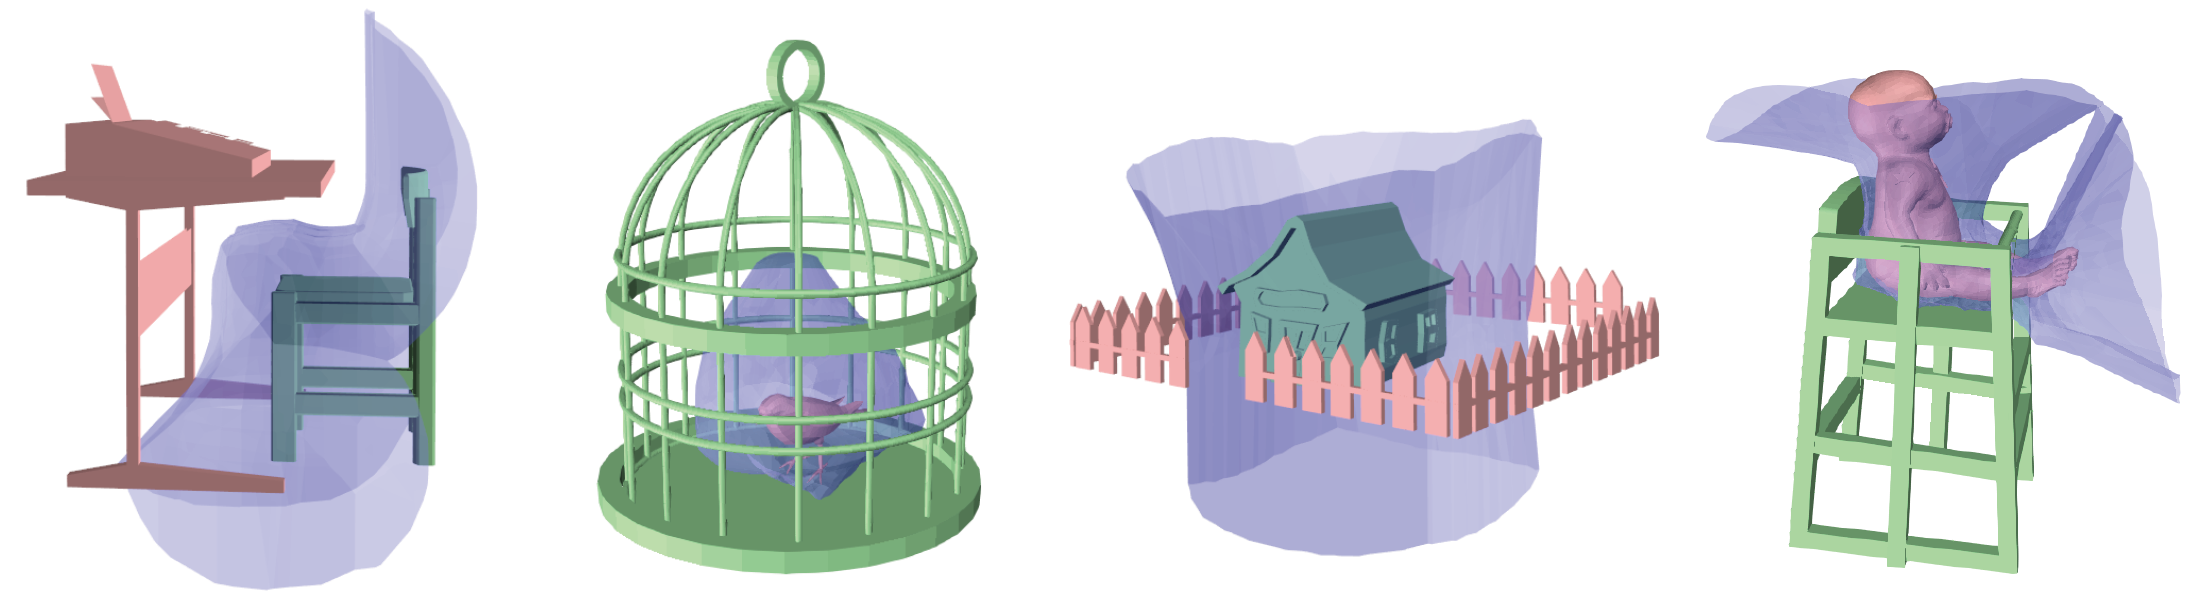
\includegraphics[width=0.99\linewidth]{fig/img/zhao_tog14_ibs}
    %\vspace{-0.2cm}
    \caption{
    The interaction bisector surface (in blue) of several two-object scenes~\cite{Zhao:2014:ISU}.
    }
    \label{fig:zhao_tog14_ibs}
\end{figure}


\paragraph*{Challenges and opportunities.}
The topic of 3D scene analysis is quite new and there are many open problems and opportunities for future.
The \emph{first} problem is an efficient way for characterizing spatial relationship.
Currently, most methods work with bounding box representation which is, albeit efficient to process,
not sufficiently informative to characterize object interaction.
For example, it is not reliable to determine the object enclosure relationship based on bounding box.
Recently, He et al.~\shortcite{Zhao:2014:ISU} propose to use biologically-inspired bisector surface to characterize the
geometric interaction between adjacent objects and index 3D scenes (Figure~\ref{fig:zhao_tog14_ibs}).
%
\emph{Secondly}, most analyses rely on the availability of object labels, given the fact that the structural layout
of scenes is mostly loose and spatial relationship is not always easy to be characterized geometrically.
This is quite restrictive since most scene models from the web do not possess reliable object tag.
Therefore, finding more powerful feature to characterize scenes and achieving tag-free analysis become indispensable.
%
\emph{Finally}, the popularity of commodity RGBD cameras has significantly simplified the acquisition
of indoor scenes. Such newly emerged scanning technique brings about new problems for scene analysis, such as online scene analysis
for high fidelity scanning and reconstruction. On the other hand, the calibrated image and depth data
help to related 3D scenes with images, enabling bidirectional transfer of information such as labels, texture, etc.

